\chapter{Existing Environments}
\label{sec:environments}

To get an idea of how others have designed a multi agent system, we will take a look on NetLogo.\\

\section{NetLogo}
NetLogo is a widespread environment for programming a MAS. NetLogo developed by Uri Wilensky in 1999, at the Northwestern University \cite{misc:northwestern}.\\ 
\indent NetLogo features a very easy programming language for both creating agents and defining environments, NetLogo also provides a way of manipulating the cosmetics of the MAS simulation. NetLogo has the advantages that even though the programming language is simple, it is also rich on features, and can create MASes that can simulate almost any possible scenario, right from advanced traffic scenarios to how many tadpoles will survive the first week of their lives. \cite{misc:netlogolib} \\
\\
The code shown in the following code-snippet, will generate a simple test with color mixing, to simulate passing of genes.

\begin{NetLogo}{This is a NetLogo source code example.}{}
to setup
  clear-all
  ask patches
    [ set pcolor (random colors) * 10 + 5
        if pcolor = 75  ;; 75 is too close to another color so change it to 125
          [ set pcolor 125 ] ]
  reset-ticks
end

to go
  ask patches [ set pcolor [pcolor] of one-of patches ]
  tick
end


; Copyright Uri Wilensky. All rights reserved.
\end{NetLogo}

This example will, together with the NetLogo GUI, create the simulation shown in \ref{fig:NetLogoscreen}. The simulation data is saved in NetLogos custom file format, so that they can be run by someone else.

\begin{figure}[H]
\begin{center}
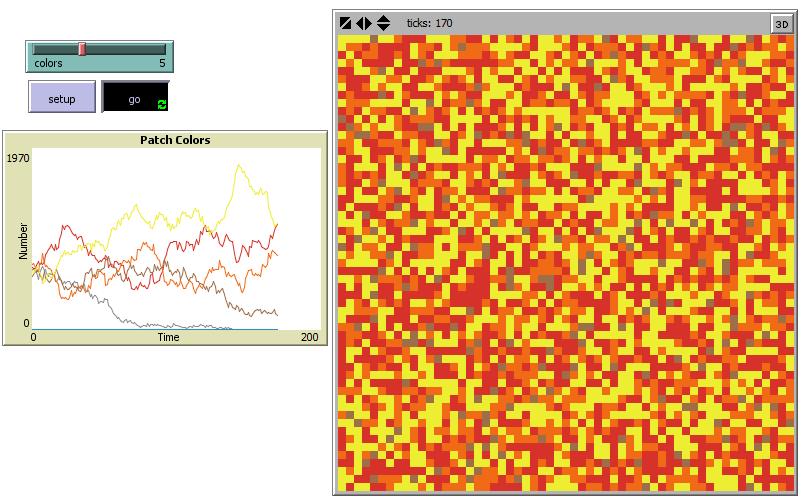
\includegraphics[scale=0.6]{Images/NetLogo.png}%
\end{center}
\caption{Simple Netlogo Simulation}%
\label{fig:NetLogoscreen}%
\end{figure}

%One example of a MAS is the NetLogo application \cite{misc:netlogo}.\\